

%%
%%%%%%%%%%%% Coloring: Rework ILU example, mention limitations
%%






\begin{frame}[fragile]
\frametitle{Parallel ILU}

  \begin{minipage}{0.5\textwidth}
    \begin{block}{ILU - Basic Idea}
      \begin{itemize}
        \item Factor sparse matrix $\matrix A \approx \tilde{\matrix L} \tilde{\matrix U}$
        \item $\tilde{\matrix L}$ and $\tilde{\matrix U}$ sparse, triangular
        \item ILU0: Pattern of $\tilde{\matrix L}$, $\tilde{\matrix U}$ equal to $\matrix A$
        \item ILUT: Keep $k$ elements per row
      \end{itemize}
    \end{block}
  \end{minipage}
%
  \begin{minipage}{0.45\textwidth}
    \begin{block}{Solver Cycle Phase}
      \vspace*{-0.1cm}
      \begin{itemize}
        \item Residual correction ${\color{red}\tilde{\matrix L}} \tilde{\matrix U} x = z$
        \item Forward solve ${\color{red}\tilde{\matrix L}} y = z$
        \item Backward solve $\tilde{\matrix U} x = y$
        \item Little parallelism in general
      \end{itemize}
    \end{block}
  \end{minipage}


  \begin{align*} 
   \left(
   \begin{array}{ccccccccc}
     \textstyle 5 &  \textstyle \times & \textstyle \times     & \textstyle \times  &   & \textstyle \times     & \textstyle \times &   &   \\
     \textstyle \color{red} \times & \textstyle 3 & \textstyle \times      &    &   &      &   &  &   \\
    \textstyle \color{red} \times & \textstyle \color{red} \times & \textstyle 4     & \textstyle \times  &   &       &   &   &   \\
%
    \textstyle \color{red} \times &   &  \textstyle\color{red}  \times     & \textstyle 5  & \textstyle \times & \textstyle \times     &   &   & \textstyle \times \\
      &   &       & \textstyle \color{red} \times  & \textstyle 5 & \textstyle \times     &   & \textstyle \times & \textstyle \times \\
    \textstyle \color{red} \times &   &      & \textstyle \color{red} \times  & \textstyle \color{red} \times & \textstyle 6     & \textstyle \times & \textstyle \times &  \\
%
    \textstyle \color{red} \times &  &       &    &   & \textstyle\color{red}  \times     & \textstyle 3 &   &   \\
      &   &       &    & \textstyle\color{red}  \times & \textstyle \color{red} \times    &   & \textstyle 4 & \textstyle \times \\
      &   &      & \textstyle\color{red}  \times  & \textstyle \color{red} \times &      &   & \textstyle \color{red} \times & \textstyle 4 \\
   \end{array}
         \right)
  \end{align*}

 
\end{frame}





\begin{frame}[fragile]
\frametitle{Parallel ILU}

     \begin{block}{ILU Level Scheduling}
      \begin{itemize}
        \item Build dependency graph
        \item Substitute as many entries as possible simultaneously
        \item Trade-off: Each step vs. multiple steps in a single kernel
      \end{itemize}

      \begin{center}
    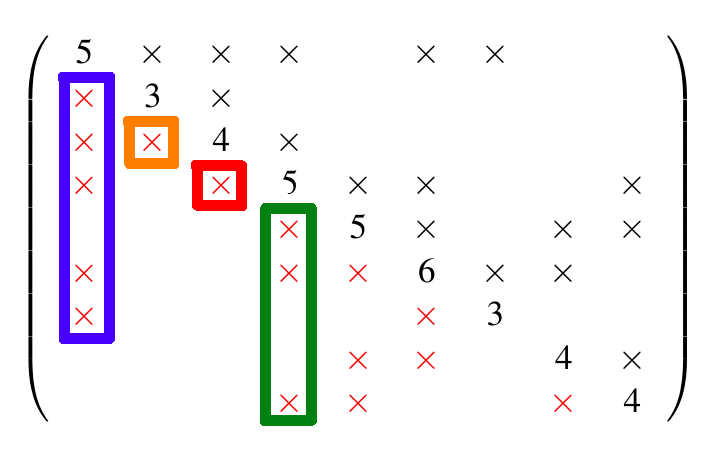
\includegraphics[width=0.65\textwidth]{figures/level-scheduling-3.png}
      \end{center}

    \end{block}
\end{frame}


\begin{frame}[fragile]
\frametitle{Parallel ILU}

     \begin{block}{ILU Interpretation on Structured Grids}
      \begin{itemize}
        \item 2d finite-difference discretization
        \item Substitution whenever all neighbors with smaller index computed
        \item Works particularly well in 3d
      \end{itemize}

      \begin{center}
    \only<1>{\hspace*{-0.17cm}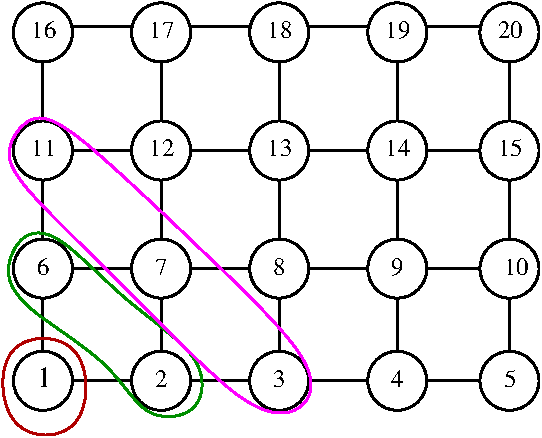
\includegraphics[width=0.4\textwidth]{figures/2d-grid-3}\hspace*{1.0cm}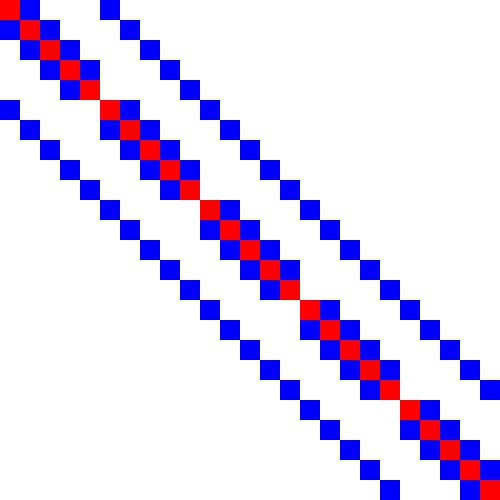
\includegraphics[width=0.4\textwidth]{figures/order_lexi}}
%
    \only<2>{\hspace*{-0.425cm}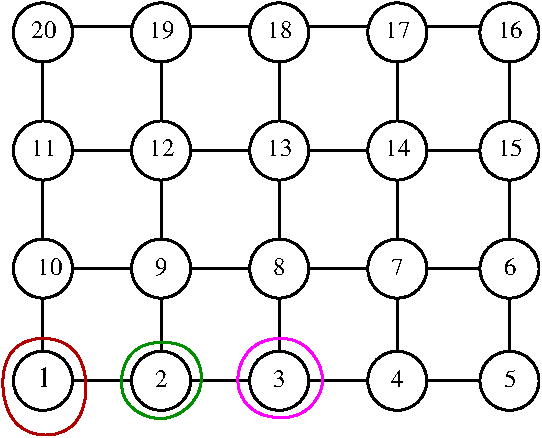
\includegraphics[width=0.4\textwidth]{figures/2d-grid-3-bad}\hspace*{1.0cm}
\includegraphics[width=0.4\textwidth]{figures/order_bad}}
%
    \only<3>{\hspace*{-0.68cm}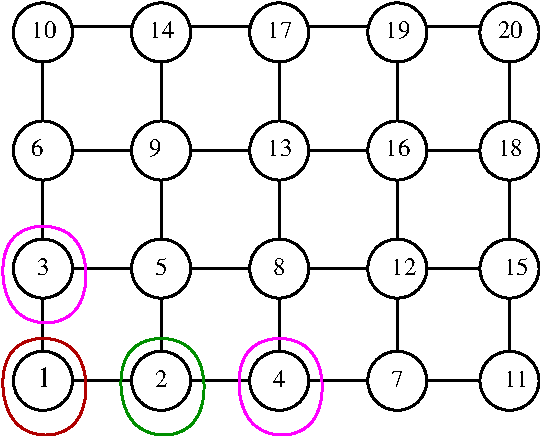
\includegraphics[width=0.4\textwidth]{figures/2d-grid-3-min}\hspace*{1.0cm}
\includegraphics[width=0.4\textwidth]{figures/order_min}}
%
    \only<4>{\hspace*{-0.75cm}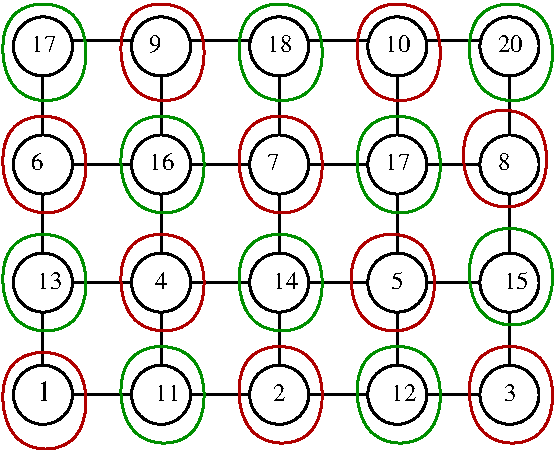
\includegraphics[width=0.41\textwidth]{figures/2d-grid-3-rb}\hspace*{0.9cm}
\includegraphics[width=0.4\textwidth]{figures/order_rb}}
      \end{center}

    \end{block}
\end{frame}



\begin{frame}[fragile]{Parallel ILU}

\begin{minipage}{0.45\textwidth}
  Sequential \\
  \lstinline|for i=2..n| \\
  \lstinline|  for k=1..i-1, (i,k) in A| \\
  \hspace*{0.7cm}$a_{ik} =  a_{ik}/a_{kk}$ \\
  \hspace*{0.7cm}\lstinline|for j=k+1..n, (i,j) in A| \\
  \hspace*{1cm}$u_{ij} =  a_{ij} - a_{ik}a_{kj}$ \\
\end{minipage} \hfill
\begin{minipage}{0.5\textwidth}
  Parallel \\
  \lstinline|for (sweep = 1, 2, ...)| \\
  \lstinline|  parallel for (i,j) in A| \\
  \lstinline|    if (i > j)| \\ 
  \hspace*{1cm}$l_{ij} =  (a_{ij} - \sum_{k=1}^{j=1} l_{ik}u_{kj}) / u_{jj}$ \\
  \lstinline|    else| \\
  \hspace*{1cm}$u_{ij} =  a_{ij} - \sum_{k=1}^{=1} l_{ik}u_{kj}$
\end{minipage}


  \begin{block}{Fine-Grained Parallel ILU Setup}
   \begin{itemize}
    \item Proposed by Chow and Patel (SISC, vol.~37(2)) for CPUs and MICs
    \item Massively parallel (one thread per row)
   \end{itemize}
  \end{block}
  
  %\pause
  
  \begin{block}{Preconditioner Application}
   \begin{itemize}
    \item Truncated Neumann series:
     \begin{align*} \mathbf{L}^{-1} \approx \sum_{k=0}^K (\mathbf{I} - \mathbf{L})^k, \quad \mathbf{U}^{-1} \approx \sum_{k=0}^K (\mathbf{I} - \mathbf{U})^k \end{align*}
    \item Exact triangular solves not necessary
   \end{itemize}
  \end{block}

\end{frame}


\begin{frame}{Parallel ILU}
  \begin{center}
    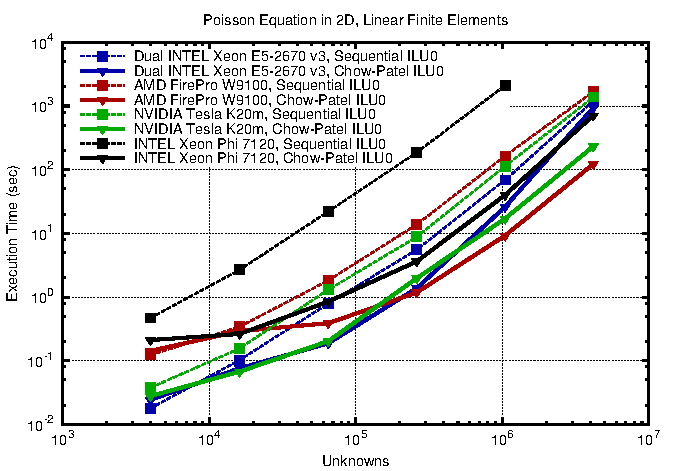
\includegraphics[width=0.95\textwidth]{ilu-2d-4}
  \end{center}
\end{frame}
